\documentclass{article}
\usepackage[utf8]{inputenc}
\usepackage{array,multirow,graphicx}
\usepackage{amsmath,amssymb,latexsym}
\usepackage{mathabx}
\usepackage{parskip}
\usepackage{listings}
\usepackage[section]{placeins}
\usepackage{hyperref}
\usepackage[english]{babel}
\usepackage{biblatex}
\renewcommand{\sfdefault}{ptm}
\graphicspath{ {/} }

\title{Report.3.SELECT}
\author{Linh Duong}
\date{November 2017}

\begin{document}

\maketitle

\section{All info of all employees}
\begin{lstlisting}[language=sql]
	select * from employees;
\end{lstlisting}
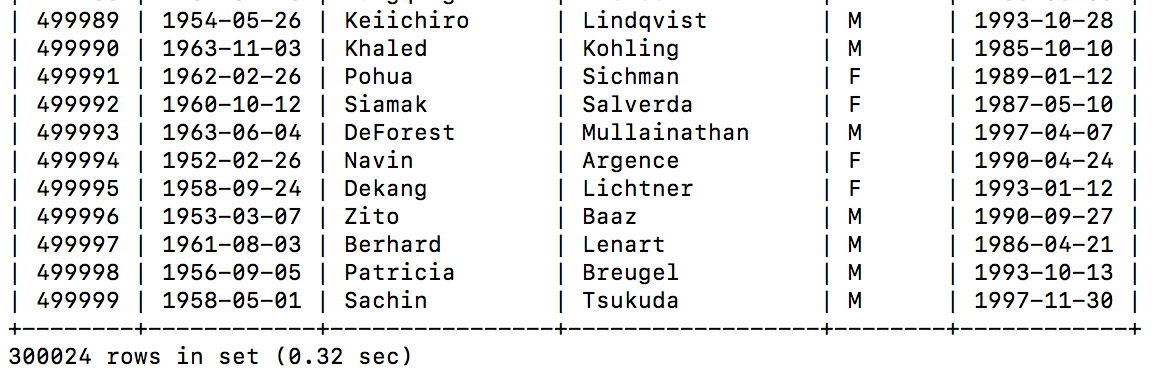
\includegraphics[width=\linewidth]{out1.png}

\section{All info of all departments}
\begin{lstlisting}[language=sql]
	select * from departments;
\end{lstlisting}
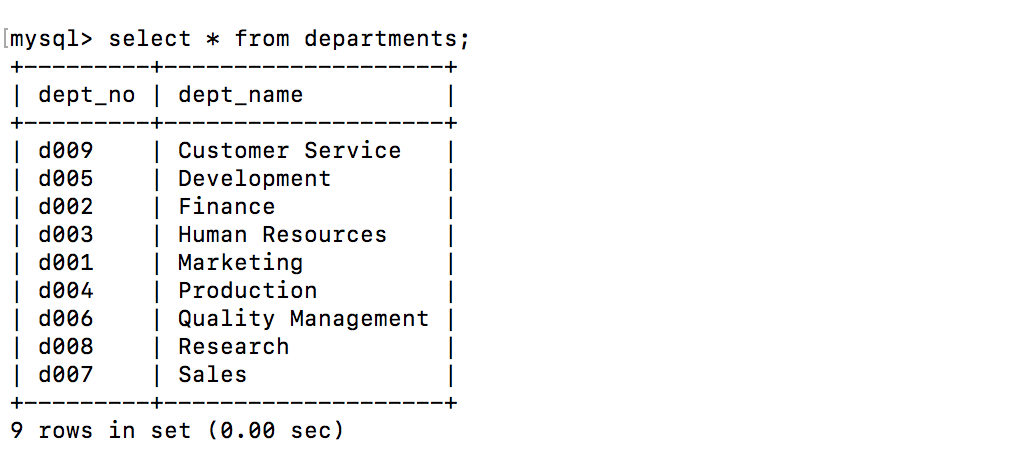
\includegraphics[width=\linewidth]{out2.png}

\section{Full names of all employees}
\begin{lstlisting}[language=sql]
	select concat(first_name,' ',last_name) as fullname 
	from employees;
\end{lstlisting}
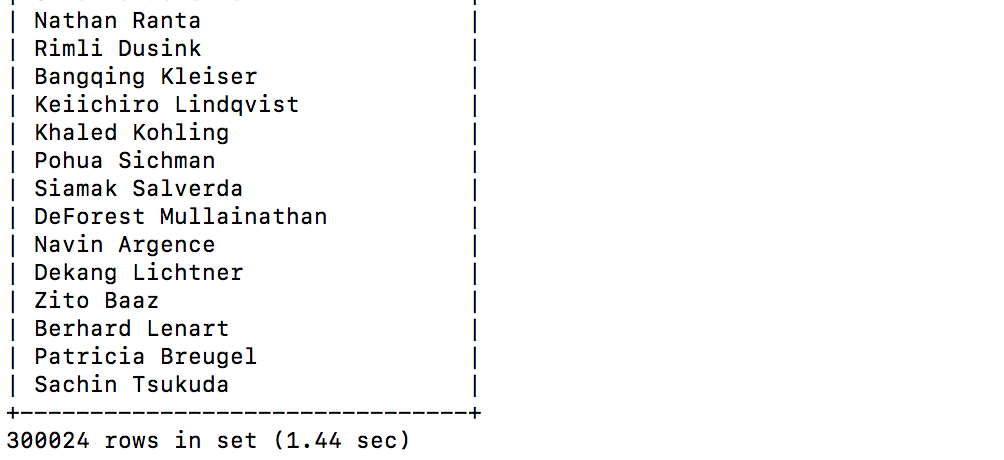
\includegraphics[width=\linewidth]{out3.png}

\section{Names of all departments}
\begin{lstlisting}[language=sql]
	select dept_name from departments;
\end{lstlisting}
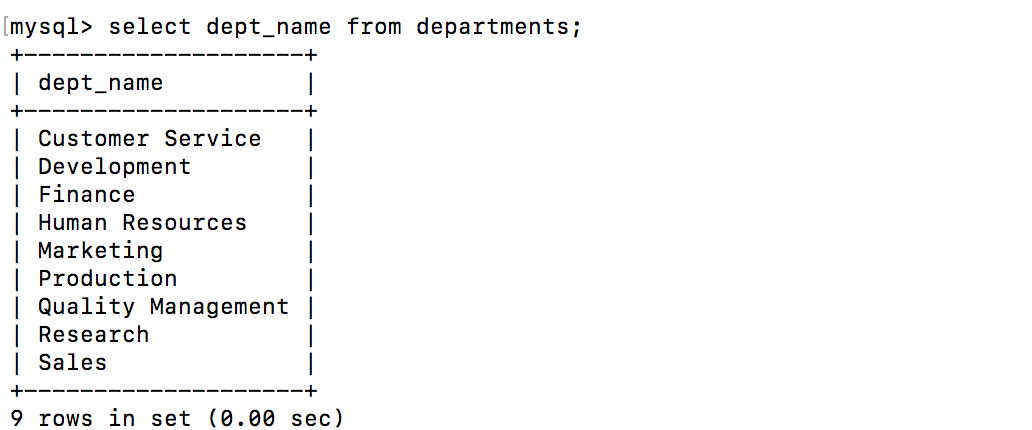
\includegraphics[width=\linewidth]{out4.png}

\section{Full names of employees working in Sales department}
\begin{lstlisting}[language=sql]
select distinct concat(first_name,' ',last_name) as fullname 
from employees 
join dept_emp on employees.emp_no = dept_emp.emp_no 
join departments on dept_emp.dept_no = departments.dept_no
where dept_name = 'Sales';
\end{lstlisting}
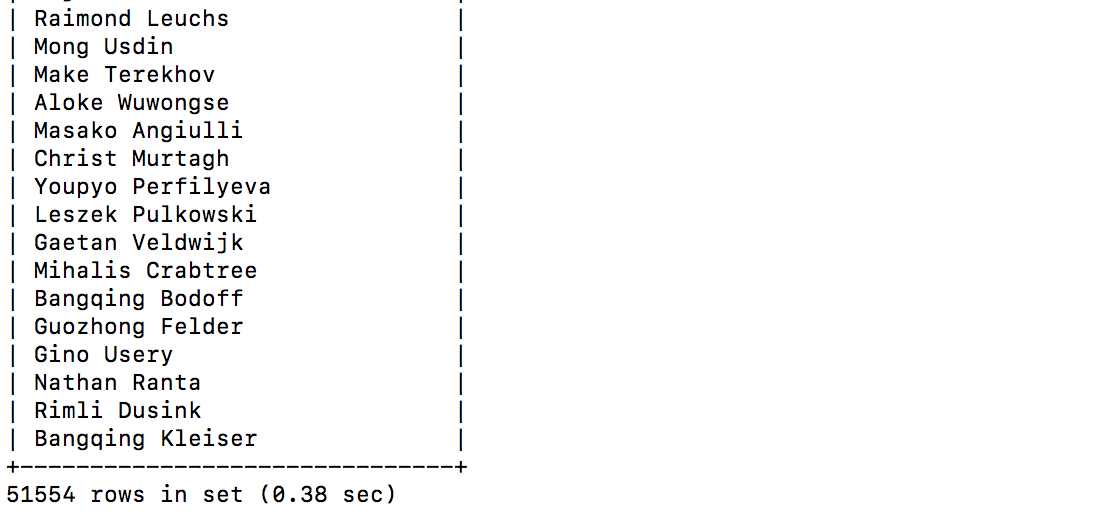
\includegraphics[width=\linewidth]{out5.png}

\section{Full names of male employees working in Finance department}
\begin{lstlisting}[language=sql]
select distinct concat(first_name,' ',last_name) as fullname 
	from employees 
	join dept_emp on employees.emp_no = dept_emp.emp_no 
	join departments on dept_emp.dept_no = departments.dept_no
	where gender ='M' and dept_name = 'Finance';
\end{lstlisting}
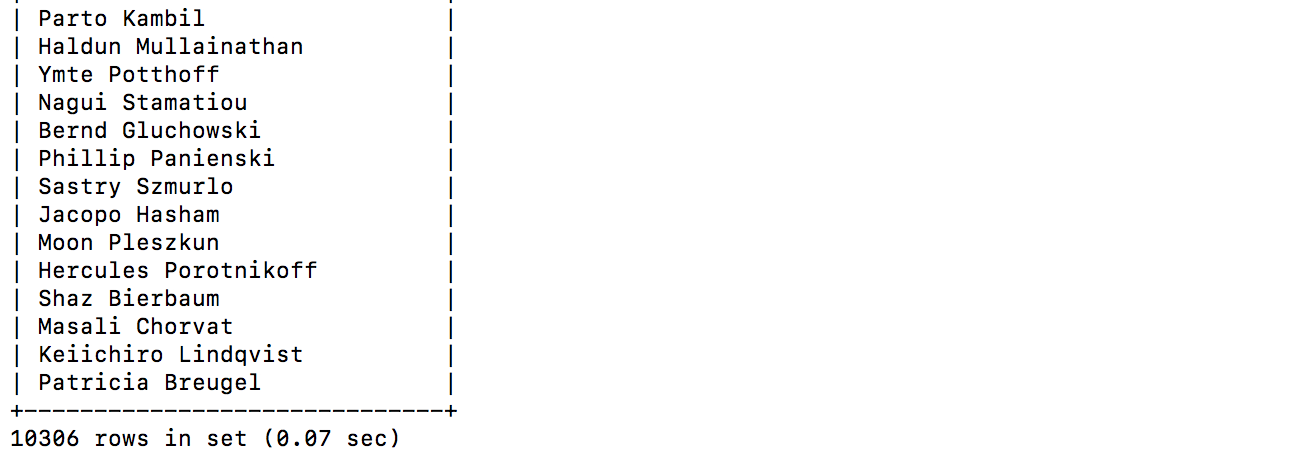
\includegraphics[width=\linewidth]{out6.png}

\section{Salaries of female employees working in Marketing department}
\begin{lstlisting}[language=sql]
select distinct salary from salaries 
join employees on salaries.emp_no = employees.emp_no 
join dept_emp on employees.emp_no = dept_emp.emp_no 
join departments on dept_emp.dept_no = departments.dept_no
where gender ='F' and dept_name = 'Marketing';
\end{lstlisting}
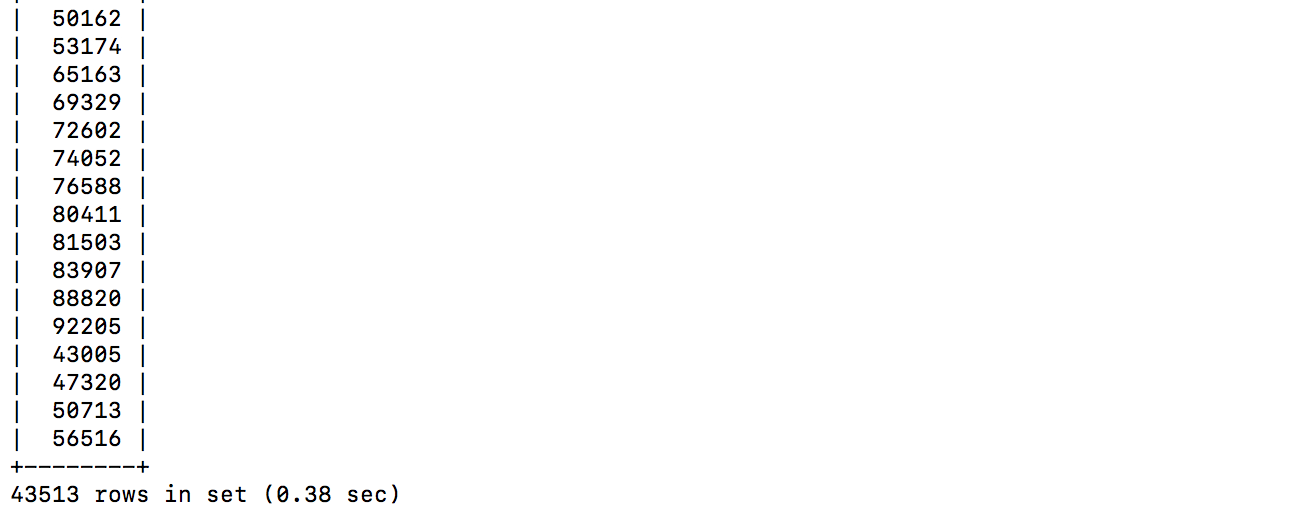
\includegraphics[width=\linewidth]{out7.png}

\section{Full names of employees who have the same last name as their manager}
\begin{lstlisting}[language=sql]
select concat(first_name,' ',employees.last_name) as fullname
from employees 
join dept_emp on dept_emp.emp_no = employees.emp_no
join (select dept_no, last_name from employees 
    join dept_manager on employees.emp_no = dept_manager.emp_no) 
as manager on manager.dept_no = dept_emp.dept_no
where employees.last_name = manager.last_name;
\end{lstlisting}
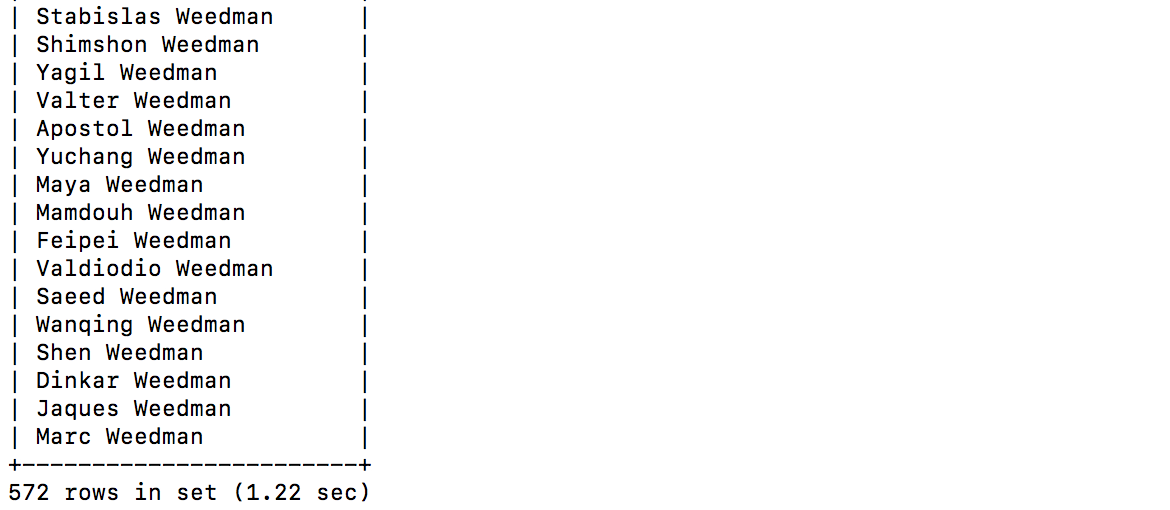
\includegraphics[width=\linewidth]{out8.png}

\section{Full names of managers who have been doing the job at least twice}
\begin{lstlisting}[language=sql]
select distinct concat(first_name,' ',last_name) as fullname, 
count(dept_manager.emp_no) as num
from employees 
join dept_manager on employees.emp_no = dept_manager.emp_no 
group by fullname having num >=2;
\end{lstlisting}
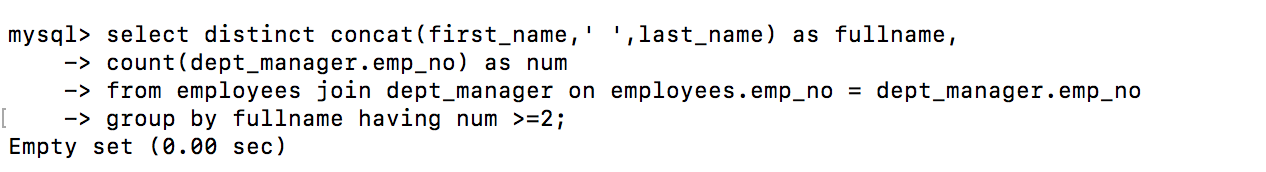
\includegraphics[width=\linewidth]{out9.png}

\section{Full names of employees who was paid more than \$100000}
\begin{lstlisting}[language=sql]
select distinct concat(first_name,' ',last_name) as fullname 
from employees 
join salaries on employees.emp_no = salaries.emp_no
where salary>100000;
\end{lstlisting}
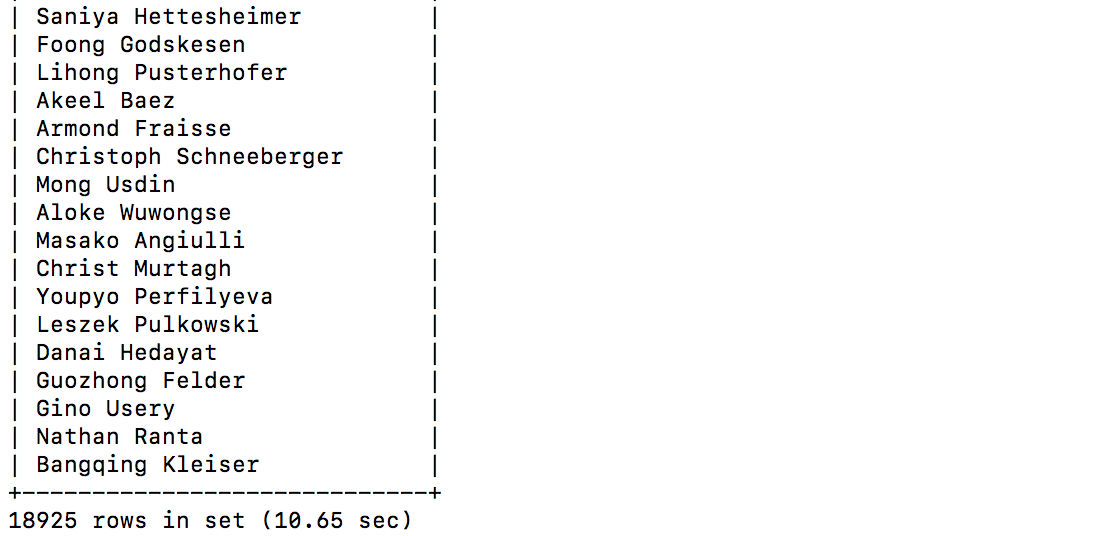
\includegraphics[width=\linewidth]{out10.png}

\section{Names of all departments that have employees paid more than \$100000}
\begin{lstlisting}[language=sql]
select distinct dept_name 
from dept_emp 
join departments on dept_emp.dept_no = departments.dept_no 
join salaries on dept_emp.emp_no = salaries.emp_no
where salary>100000;
\end{lstlisting}
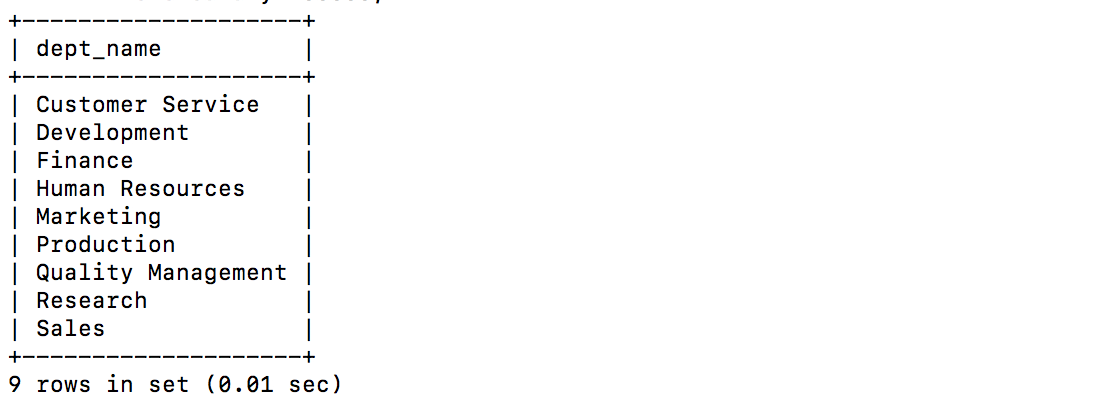
\includegraphics[width=\linewidth]{out11.png}


\end{document}
